\chapter{Understanding Desire}

This chapter follows J. Krishnamurti in dialogue with Dr. Alan W. Anderson, using source material credited to J. Krishnamurti and the Krishnamurti Foundation Trust, with course curation by LazyingArt LLC through Video2Book. The conversation is not a blackboard lecture, so the mathematical notation below is deliberately modest: it is a compact way of tracking distinctions, movements, and substitutions in the inquiry. We will keep the spoken order: fear, freedom, pleasure, desire, control, and finally the unresolved opening toward joy.

\section{Fear, Pleasure, And Freedom}

Anderson begins where the previous conversation left off. Fear and pleasure had been described as opposite sides of the same coin, and the natural impulse is to move from fear into pleasure. Krishnamurti pauses before doing that. Fear is not merely a private feeling; it has generated misery, ideologies, beliefs, gods, and activities that keep human beings from being completely free.

The first serious distinction is therefore not about pleasure, but about freedom. We commonly say that one wants freedom from fear, freedom from conflict, freedom from burden. Anderson even tests the related phrase ``freedom for.'' Krishnamurti's answer is precise: ``from'' and ``for'' still imply direction, opposition, and conflict. They are not the same as freedom itself.

Let \(F\) denote freedom itself. Let \(F_{\mathrm{from}}(x)\) denote the movement of escape from some object \(x\), and let \(F_{\mathrm{for}}(x)\) denote movement toward an intended end. The distinction can be held in the following shorthand:
\begin{equation}
F_{\mathrm{from}}(x) \neq F,
\qquad
F_{\mathrm{for}}(x) \neq F.
\end{equation}
The notation is not a definition of freedom. It is a guardrail. It prevents us from confusing freedom with a reaction against something that still governs the field.

\subsection{Question \& Answer}

\paragraph{Question.}
If one is free from fear, is that not freedom?

\paragraph{Answer.}
Not in the full sense Krishnamurti is pointing to. If fear remains the object from which one is escaping, then fear still organizes the movement. Freedom is not a project of throwing burdens away. It is closer to the ending of the burden as a fact. That is why the conversation also rejects ``freedom in'' something. The preposition itself keeps suggesting a location, an object, or a goal.

\section{Pleasure Without Condemnation}

Only after this clearing does the dialogue return to pleasure. Pleasure and fear are said to be deeply rooted in us. They cannot really be separated in life, but for the sake of investigation they can be looked at distinctly. Anderson hears the pattern immediately: punishment and reward, fear and pleasure, the anxiety of not receiving what one anticipates.

We can keep that pairing compactly:
\begin{equation}
\mathrm{Fear} \leftrightarrow \mathrm{Pleasure},
\qquad
\mathrm{Punishment} \leftrightarrow \mathrm{Reward}.
\end{equation}
The double arrow does not state a mechanical law. It marks the way the lecture pairs these principles. Where reward becomes central, punishment is nearby; where pleasure becomes central, fear is not far away.

Before looking at pleasure, Krishnamurti removes the usual moral reflexes. We are not condemning pleasure. We are not justifying it. We are not becoming puritanical, and we are not becoming permissive. We are trying to observe the structure and nature of pleasure as fear had been observed.

\begin{definition}
In this chapter, \emph{observation} means looking without condemnation, justification, acceptance, or suppression. It is not a technique applied to desire; it is the clarity without which desire cannot be seen.
\end{definition}

This is an important pacing point. The lecture does not rush to say what pleasure is. It first prepares the quality of looking.

\section{Why Pleasure Sends Us Back To Desire}

Anderson names the ordinary field of pleasure: anticipation, gratification, satisfaction, and fulfilment. Krishnamurti accepts the direction, but he does not yet analyze pleasure directly. To understand pleasure, he says, one has first to look into desire.

The motivation for this turn is social as well as inward. Desire is not left alone. It is stimulated by commercialism, consumerism, propaganda, fashion, and the promise of more. Krishnamurti's examples are ordinary: the appeal of possessions, the excitement of acquisition, the sense that two are not enough when twelve can be had. Anderson adds that pleasure fades and therefore requires a stronger stimulus the next time.

A compact reconstruction of this movement is
\begin{equation}
\mathrm{stimulation}
\longrightarrow D
\longrightarrow \mathrm{fulfilment}
\longrightarrow \mathrm{fading}
\longrightarrow \mathrm{stronger\ stimulation}.
\end{equation}
Here \(D\) denotes desire. This is not an economic theory. It is a note-taking form of the sequence described in the conversation: desire is nourished, expanded, and inflamed by a world that profits from its continuation.

The same structure appears in ritual. Words, chants, symbols, images, flowers, incense, color, and ceremonial beauty can all be stimulating. Krishnamurti does not deny their beauty. The question is whether one is listening to what is being said, or whether one is being carried by the pleasure of how it is said. Anderson recognizes the same problem in teaching: students may attend to the recitation and miss the meaning.

\section{Appetite, Desire, And The Object}

Anderson next asks about appetite. Is desire like hunger? Is appetite natural while desire is artificial? Krishnamurti does not separate them that sharply. Appetite and desire are related. There is physical appetite, psychological appetite, sexual appetite, intellectual appetite, and an appetite for ritual. The point of this list is not classification for its own sake. It prepares the crucial distinction between the object desired and the movement of desire.

Let \(O_i\) denote an object of desire. It may be a coat, a house, a car, knowledge, God, enlightenment, sex, power, ritual, or comfort. The lecture's reduction is:
\begin{equation}
O_i \ \hbox{varies},
\qquad
D \ \hbox{remains}.
\end{equation}
The mind may call one object noble and another ignoble, but the naming does not change the movement. The object varies according to conditioning, tendency, circumstance, and culture. Desire as a movement is what Krishnamurti wants to see.

\begin{table}
\centering
\begin{tabular}{p{0.25\linewidth}p{0.30\linewidth}p{0.32\linewidth}}
Object field & Typical stimulus & Movement emphasized \\
Possession & coat, tie, house, car & acquisition and ownership \\
Knowledge & discussion, comparison & accumulation and subtle competition \\
Ritual & chant, symbol, image & stimulation and repetition \\
God or truth & ideal, path, authority & transfer to a higher object \\
Power & security, future fulfilment & control in order to secure pleasure
\end{tabular}
\end{table}

The table is only a pocket map. It should not harden into a theory. Its use is to keep visible the lecture's refrain: the object changes, but the movement must be watched.

\section{The Process Of Desire}

The question now becomes direct: what is desire? Anderson proposes one possible route: perhaps desire is a sense of absence. Krishnamurti refuses that abstraction at this point. He is not asking for a speculative definition; he is asking how desire comes about in us.

The transcript gives the process twice, with a slight variation. Krishnamurti first says visual perception, sensation, contact, and desire. Anderson then recaps it as visual perception, contact, sensation, desire. To avoid false precision, we keep contact and sensation together:
\begin{equation}
\mathrm{visual\ perception}
\longrightarrow
\mathrm{contact/sensation}
\longrightarrow
D.
\end{equation}
If desire is frustrated, Anderson says, anger follows. Krishnamurti agrees that all the rest follows:
\begin{equation}
D + \mathrm{frustration}
\longrightarrow
\mathrm{anger\ and\ further\ reaction}.
\end{equation}

\subsection{Question \& Answer}

\paragraph{Question.}
Is desire basically a sense of absence?

\paragraph{Answer.}
Krishnamurti does not answer by defining desire as lack. He asks us to see its arising. There is perception; there is contact and sensation; desire comes out of that movement. The difference matters. A theory of absence can become another explanation held at a distance, while the lecture is asking for observation of the movement itself.

\begin{figure}
\centering
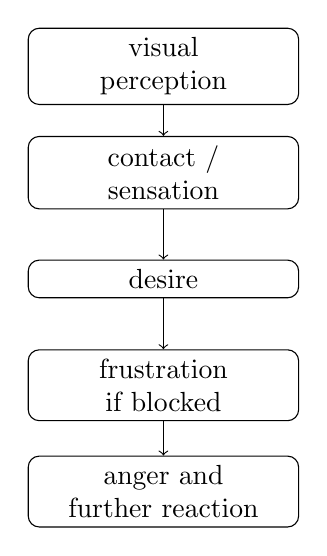
\begin{tikzpicture}
\node[draw, rounded corners, align=center, text width=3.2cm] (a) at (0,0) {visual\\perception};
\node[draw, rounded corners, align=center, text width=3.2cm] (b) at (0,-1.35) {contact /\\sensation};
\node[draw, rounded corners, align=center, text width=3.2cm] (c) at (0,-2.70) {desire};
\node[draw, rounded corners, align=center, text width=3.2cm] (d) at (0,-4.05) {frustration\\if blocked};
\node[draw, rounded corners, align=center, text width=3.2cm] (e) at (0,-5.40) {anger and\\further reaction};
\draw[->] (a) -- (b);
\draw[->] (b) -- (c);
\draw[->] (c) -- (d);
\draw[->] (d) -- (e);
\end{tikzpicture}
\end{figure}

This figure is a transcript-based schematic. It is not a drawing from a board. Its value is that it keeps the inquiry narrow and sequential: perception, contact and sensation, desire, frustration, reaction.

\section{Control And The Loss Of Free Energy}

Once desire has been seen in outline, the inherited answer appears: control it, suppress it, or transfer it to something higher. Religious discipline says, in effect: desire dissipates energy; therefore hold it, master it, redirect it toward God, truth, or enlightenment. Krishnamurti gives concrete images: the person who keeps looking at a sacred book so as not to see what attracts him; the monks who do not look at sky, trees, water, or passers-by; a life bent toward avoiding temptation.

The lecture's reversal is severe. Control is not freedom from desire. Control is part of the same field of fear and desire. It narrows perception, organizes avoidance, and turns discipline into suppression. The shorthand is:
\begin{equation}
D
\xrightarrow{\mathrm{control/suppression/transfer}}
\mathrm{restriction}
+
\mathrm{loss\ of\ free\ energy}.
\end{equation}
The phrase ``free energy'' is not a physical term here. It names the vitality and openness that are squeezed out when the mind is occupied with controlling itself.

\subsection{Question \& Answer}

\paragraph{Question.}
Need there be control of desire at all?

\paragraph{Answer.}
That is the problem Krishnamurti says now arises. The usual answer is control, but control assumes an inner division: one part of the mind will dominate another. That division is already conflict. So the question is not how to control desire more effectively; the question is whether desire can be understood without setting up the controller.

\begin{figure}
\centering
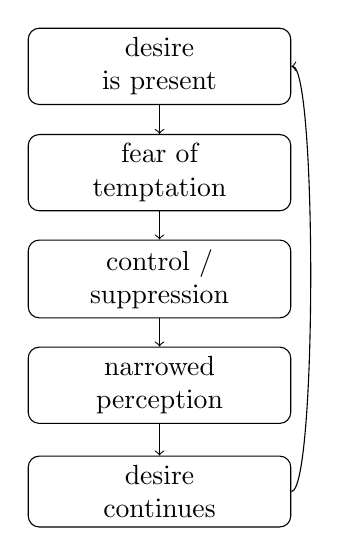
\begin{tikzpicture}
\node[draw, rounded corners, align=center, text width=3.1cm] (a) at (0,0) {desire\\is present};
\node[draw, rounded corners, align=center, text width=3.1cm] (b) at (0,-1.35) {fear of\\temptation};
\node[draw, rounded corners, align=center, text width=3.1cm] (c) at (0,-2.70) {control /\\suppression};
\node[draw, rounded corners, align=center, text width=3.1cm] (d) at (0,-4.05) {narrowed\\perception};
\node[draw, rounded corners, align=center, text width=3.1cm] (e) at (0,-5.40) {desire\\continues};
\draw[->] (a) -- (b);
\draw[->] (b) -- (c);
\draw[->] (c) -- (d);
\draw[->] (d) -- (e);
\draw[->] (e.east) .. controls (2.0,-5.40) and (2.0,0) .. (a.east);
\end{tikzpicture}
\end{figure}

This loop is the danger in the traditional solution. Control may appear to oppose desire, but it can also keep desire in motion by making the whole mind revolve around avoidance.

\begin{proposition}
If desire is merely transferred from one object to another, the movement of desire has not ended.
\end{proposition}

\begin{proof}
Let \(O_{\mathrm{worldly}}\) denote an object such as money, possession, status, or comfort. Let \(O_{\mathrm{spiritual}}\) denote an object such as God, truth, enlightenment, or heaven. If the object changes but the movement \(D\) remains a movement of acquisition, fulfilment, becoming, or security, then the substitution is structural rather than transformative:
\begin{equation}
D(O_{\mathrm{worldly}})
\sim
D(O_{\mathrm{spiritual}}).
\end{equation}
The symbol \(\sim\) marks similarity of movement, not formal equality. The lecture's conclusion is practical: changing the object does not by itself resolve desire.
\end{proof}

\section{The Cruelty Of Substitution}

The conversation now becomes concrete, and it should remain concrete. Krishnamurti speaks of serious monks whose lives were organized around controlling desire. They avoided beauty because beauty might become temptation. He tells of a young monk who had taken a vow of celibacy and acted violently upon his own body in the name of controlling sexual appetite. Anderson brings in Origen as a parallel case. Krishnamurti then widens the point: many have tortured themselves for an idea, a symbol, a concept.

These examples are not included for sensation. They show the cost of taking an idea for reality. The phrase ``God,'' ``truth,'' or ``enlightenment'' may become an object around which desire organizes itself. The language changes; the movement may not.

A second set of examples deepens the point. One man spends twenty-five years meditating on truth and later sees that he has been caught in a verbal and intellectual structure. Another spends fifty-five years going from teacher to teacher in search of God, only to return with nothing. Krishnamurti places this beside the business life: fifty years going to the office in pursuit of money and things. The contrast is sharp, but the structure may be identical.

We can write the comparison as
\begin{align}
\mathrm{money,\ things,\ status} &\longrightarrow D,\\
\mathrm{God,\ truth,\ enlightenment} &\longrightarrow D.
\end{align}
The notation is intentionally spare. It does not equate money with truth. It says that desire can attach to either field.

From here the lecture asks the practical question that the stories have prepared: how is one to live with desire? Desire is there. The moment there is seeing, beauty, scent, contact, admiration, enjoyment, the movement can begin. The question is whether one can live without the old machinery of control.

\section{Pleasure, Enjoyment, And Joy}

Only now does the dialogue return to pleasure in earnest. The foundation has been laid: unless appetite and desire are understood, pleasure cannot be understood deeply. Fear and pleasure remain active principles, comparable to punishment and reward.

There is another important turn. Anderson asks whether the search for power is the attempt to secure a pleasure not yet realized. Krishnamurti agrees. The attempt to negate desire through power is itself another search. The mind says: if I can control this, I will secure a future state, a future pleasure, a future safety.

Thus society seems split, but the split is not clean. The religious side says control. Commercialism says enjoy, buy, sell. The human mind moves between the two: pursue pleasure here, offer something to God there. The game continues because neither side has understood desire.

At the end of the conversation, a new vocabulary appears:
\begin{equation}
P,\quad E,\quad J,\quad H,
\end{equation}
where \(P\) is pleasure, \(E\) is enjoyment, \(J\) is joy, and \(H\) is happiness. Krishnamurti says joy is happiness, but the relation between pleasure, enjoyment, joy, and happiness is not completed in this conversation. We should therefore keep the relation open:
\begin{equation}
J \approx H,
\qquad
P \ ? \ E \ ? \ J/H.
\end{equation}
The question marks matter. The lecture is not closing with a doctrine of happiness; it is opening the next inquiry.

The final example is beauty. One sees a mountain, a lake, a single tree on a hill. At that moment, Krishnamurti says, there is nothing but that. The beauty has knocked everything out of the observer. There is no division between me and that. There is purity and enjoyment. The conversation stops at the edge of the next step: now see what takes place.

\section{Summary}

The lecture moves with unusual care. It begins from fear, not because fear is the announced topic, but because pleasure cannot be separated from fear. It then distinguishes freedom itself from the movements of escape and pursuit. It refuses condemnation and justification. It turns from pleasure to desire, from desire's objects to desire's movement, from movement to control, and from control to the possibility of living without control.

The compact map is:
\begin{align}
F_{\mathrm{from}}(x) &\neq F,
&
F_{\mathrm{for}}(x) &\neq F,\\
\mathrm{Fear} &\leftrightarrow \mathrm{Pleasure},
&
\mathrm{Punishment} &\leftrightarrow \mathrm{Reward},\\
O_i \ \hbox{varies},\quad D &\ \hbox{remains},\\
\mathrm{visual\ perception}
\to
\mathrm{contact/sensation}
&\to
D,\\
D
\xrightarrow{\mathrm{control}}
\mathrm{restriction}
&+
\mathrm{loss\ of\ free\ energy}.
\end{align}
None of this is a substitute for the inquiry itself. It is only a disciplined notation for following the movement. The next step belongs to pleasure, enjoyment, joy, and happiness; but this chapter has prepared the ground by showing that desire is not understood by condemning it, indulging it, or controlling it. It is understood, if at all, by observing its movement directly.